\documentclass{lab1-article}

\title{Equazione della catenaria}

\usepackage{fancyvrb}
\usepackage{hyperref}
\makeatletter
\def\PY@reset{\let\PY@it=\relax \let\PY@bf=\relax%
    \let\PY@ul=\relax \let\PY@tc=\relax%
    \let\PY@bc=\relax \let\PY@ff=\relax}
\def\PY@tok#1{\csname PY@tok@#1\endcsname}
\def\PY@toks#1+{\ifx\relax#1\empty\else%
    \PY@tok{#1}\expandafter\PY@toks\fi}
\def\PY@do#1{\PY@bc{\PY@tc{\PY@ul{%
    \PY@it{\PY@bf{\PY@ff{#1}}}}}}}
\def\PY#1#2{\PY@reset\PY@toks#1+\relax+\PY@do{#2}}

\expandafter\def\csname PY@tok@gd\endcsname{\def\PY@tc##1{\textcolor[rgb]{0.63,0.00,0.00}{##1}}}
\expandafter\def\csname PY@tok@gu\endcsname{\let\PY@bf=\textbf\def\PY@tc##1{\textcolor[rgb]{0.50,0.00,0.50}{##1}}}
\expandafter\def\csname PY@tok@gt\endcsname{\def\PY@tc##1{\textcolor[rgb]{0.00,0.27,0.87}{##1}}}
\expandafter\def\csname PY@tok@gs\endcsname{\let\PY@bf=\textbf}
\expandafter\def\csname PY@tok@gr\endcsname{\def\PY@tc##1{\textcolor[rgb]{1.00,0.00,0.00}{##1}}}
\expandafter\def\csname PY@tok@cm\endcsname{\let\PY@it=\textit\def\PY@tc##1{\textcolor[rgb]{0.25,0.50,0.50}{##1}}}
\expandafter\def\csname PY@tok@vg\endcsname{\def\PY@tc##1{\textcolor[rgb]{0.10,0.09,0.49}{##1}}}
\expandafter\def\csname PY@tok@m\endcsname{\def\PY@tc##1{\textcolor[rgb]{0.40,0.40,0.40}{##1}}}
\expandafter\def\csname PY@tok@mh\endcsname{\def\PY@tc##1{\textcolor[rgb]{0.40,0.40,0.40}{##1}}}
\expandafter\def\csname PY@tok@go\endcsname{\def\PY@tc##1{\textcolor[rgb]{0.53,0.53,0.53}{##1}}}
\expandafter\def\csname PY@tok@ge\endcsname{\let\PY@it=\textit}
\expandafter\def\csname PY@tok@vc\endcsname{\def\PY@tc##1{\textcolor[rgb]{0.10,0.09,0.49}{##1}}}
\expandafter\def\csname PY@tok@il\endcsname{\def\PY@tc##1{\textcolor[rgb]{0.40,0.40,0.40}{##1}}}
\expandafter\def\csname PY@tok@cs\endcsname{\let\PY@it=\textit\def\PY@tc##1{\textcolor[rgb]{0.25,0.50,0.50}{##1}}}
\expandafter\def\csname PY@tok@cp\endcsname{\def\PY@tc##1{\textcolor[rgb]{0.74,0.48,0.00}{##1}}}
\expandafter\def\csname PY@tok@gi\endcsname{\def\PY@tc##1{\textcolor[rgb]{0.00,0.63,0.00}{##1}}}
\expandafter\def\csname PY@tok@gh\endcsname{\let\PY@bf=\textbf\def\PY@tc##1{\textcolor[rgb]{0.00,0.00,0.50}{##1}}}
\expandafter\def\csname PY@tok@ni\endcsname{\let\PY@bf=\textbf\def\PY@tc##1{\textcolor[rgb]{0.60,0.60,0.60}{##1}}}
\expandafter\def\csname PY@tok@nl\endcsname{\def\PY@tc##1{\textcolor[rgb]{0.63,0.63,0.00}{##1}}}
\expandafter\def\csname PY@tok@nn\endcsname{\let\PY@bf=\textbf\def\PY@tc##1{\textcolor[rgb]{0.00,0.00,1.00}{##1}}}
\expandafter\def\csname PY@tok@no\endcsname{\def\PY@tc##1{\textcolor[rgb]{0.53,0.00,0.00}{##1}}}
\expandafter\def\csname PY@tok@na\endcsname{\def\PY@tc##1{\textcolor[rgb]{0.49,0.56,0.16}{##1}}}
\expandafter\def\csname PY@tok@nb\endcsname{\def\PY@tc##1{\textcolor[rgb]{0.00,0.50,0.00}{##1}}}
\expandafter\def\csname PY@tok@nc\endcsname{\let\PY@bf=\textbf\def\PY@tc##1{\textcolor[rgb]{0.00,0.00,1.00}{##1}}}
\expandafter\def\csname PY@tok@nd\endcsname{\def\PY@tc##1{\textcolor[rgb]{0.67,0.13,1.00}{##1}}}
\expandafter\def\csname PY@tok@ne\endcsname{\let\PY@bf=\textbf\def\PY@tc##1{\textcolor[rgb]{0.82,0.25,0.23}{##1}}}
\expandafter\def\csname PY@tok@nf\endcsname{\def\PY@tc##1{\textcolor[rgb]{0.00,0.00,1.00}{##1}}}
\expandafter\def\csname PY@tok@si\endcsname{\let\PY@bf=\textbf\def\PY@tc##1{\textcolor[rgb]{0.73,0.40,0.53}{##1}}}
\expandafter\def\csname PY@tok@s2\endcsname{\def\PY@tc##1{\textcolor[rgb]{0.73,0.13,0.13}{##1}}}
\expandafter\def\csname PY@tok@vi\endcsname{\def\PY@tc##1{\textcolor[rgb]{0.10,0.09,0.49}{##1}}}
\expandafter\def\csname PY@tok@nt\endcsname{\let\PY@bf=\textbf\def\PY@tc##1{\textcolor[rgb]{0.00,0.50,0.00}{##1}}}
\expandafter\def\csname PY@tok@nv\endcsname{\def\PY@tc##1{\textcolor[rgb]{0.10,0.09,0.49}{##1}}}
\expandafter\def\csname PY@tok@s1\endcsname{\def\PY@tc##1{\textcolor[rgb]{0.73,0.13,0.13}{##1}}}
\expandafter\def\csname PY@tok@sh\endcsname{\def\PY@tc##1{\textcolor[rgb]{0.73,0.13,0.13}{##1}}}
\expandafter\def\csname PY@tok@sc\endcsname{\def\PY@tc##1{\textcolor[rgb]{0.73,0.13,0.13}{##1}}}
\expandafter\def\csname PY@tok@sx\endcsname{\def\PY@tc##1{\textcolor[rgb]{0.00,0.50,0.00}{##1}}}
\expandafter\def\csname PY@tok@bp\endcsname{\def\PY@tc##1{\textcolor[rgb]{0.00,0.50,0.00}{##1}}}
\expandafter\def\csname PY@tok@c1\endcsname{\let\PY@it=\textit\def\PY@tc##1{\textcolor[rgb]{0.25,0.50,0.50}{##1}}}
\expandafter\def\csname PY@tok@kc\endcsname{\let\PY@bf=\textbf\def\PY@tc##1{\textcolor[rgb]{0.00,0.50,0.00}{##1}}}
\expandafter\def\csname PY@tok@c\endcsname{\let\PY@it=\textit\def\PY@tc##1{\textcolor[rgb]{0.25,0.50,0.50}{##1}}}
\expandafter\def\csname PY@tok@mf\endcsname{\def\PY@tc##1{\textcolor[rgb]{0.40,0.40,0.40}{##1}}}
\expandafter\def\csname PY@tok@err\endcsname{\def\PY@bc##1{\setlength{\fboxsep}{0pt}\fcolorbox[rgb]{1.00,0.00,0.00}{1,1,1}{\strut ##1}}}
\expandafter\def\csname PY@tok@kd\endcsname{\let\PY@bf=\textbf\def\PY@tc##1{\textcolor[rgb]{0.00,0.50,0.00}{##1}}}
\expandafter\def\csname PY@tok@ss\endcsname{\def\PY@tc##1{\textcolor[rgb]{0.10,0.09,0.49}{##1}}}
\expandafter\def\csname PY@tok@sr\endcsname{\def\PY@tc##1{\textcolor[rgb]{0.73,0.40,0.53}{##1}}}
\expandafter\def\csname PY@tok@mo\endcsname{\def\PY@tc##1{\textcolor[rgb]{0.40,0.40,0.40}{##1}}}
\expandafter\def\csname PY@tok@kn\endcsname{\let\PY@bf=\textbf\def\PY@tc##1{\textcolor[rgb]{0.00,0.50,0.00}{##1}}}
\expandafter\def\csname PY@tok@mi\endcsname{\def\PY@tc##1{\textcolor[rgb]{0.40,0.40,0.40}{##1}}}
\expandafter\def\csname PY@tok@gp\endcsname{\let\PY@bf=\textbf\def\PY@tc##1{\textcolor[rgb]{0.00,0.00,0.50}{##1}}}
\expandafter\def\csname PY@tok@o\endcsname{\def\PY@tc##1{\textcolor[rgb]{0.40,0.40,0.40}{##1}}}
\expandafter\def\csname PY@tok@kr\endcsname{\let\PY@bf=\textbf\def\PY@tc##1{\textcolor[rgb]{0.00,0.50,0.00}{##1}}}
\expandafter\def\csname PY@tok@s\endcsname{\def\PY@tc##1{\textcolor[rgb]{0.73,0.13,0.13}{##1}}}
\expandafter\def\csname PY@tok@kp\endcsname{\def\PY@tc##1{\textcolor[rgb]{0.00,0.50,0.00}{##1}}}
\expandafter\def\csname PY@tok@w\endcsname{\def\PY@tc##1{\textcolor[rgb]{0.73,0.73,0.73}{##1}}}
\expandafter\def\csname PY@tok@kt\endcsname{\def\PY@tc##1{\textcolor[rgb]{0.69,0.00,0.25}{##1}}}
\expandafter\def\csname PY@tok@ow\endcsname{\let\PY@bf=\textbf\def\PY@tc##1{\textcolor[rgb]{0.67,0.13,1.00}{##1}}}
\expandafter\def\csname PY@tok@sb\endcsname{\def\PY@tc##1{\textcolor[rgb]{0.73,0.13,0.13}{##1}}}
\expandafter\def\csname PY@tok@k\endcsname{\let\PY@bf=\textbf\def\PY@tc##1{\textcolor[rgb]{0.00,0.50,0.00}{##1}}}
\expandafter\def\csname PY@tok@se\endcsname{\let\PY@bf=\textbf\def\PY@tc##1{\textcolor[rgb]{0.73,0.40,0.13}{##1}}}
\expandafter\def\csname PY@tok@sd\endcsname{\let\PY@it=\textit\def\PY@tc##1{\textcolor[rgb]{0.73,0.13,0.13}{##1}}}

\def\PYZbs{\char`\\}
\def\PYZus{\char`\_}
\def\PYZob{\char`\{}
\def\PYZcb{\char`\}}
\def\PYZca{\char`\^}
\def\PYZam{\char`\&}
\def\PYZlt{\char`\<}
\def\PYZgt{\char`\>}
\def\PYZsh{\char`\#}
\def\PYZpc{\char`\%}
\def\PYZdl{\char`\$}
\def\PYZhy{\char`\-}
\def\PYZsq{\char`\'}
\def\PYZdq{\char`\"}
\def\PYZti{\char`\~}
% for compatibility with earlier versions
\def\PYZat{@}
\def\PYZlb{[}
\def\PYZrb{]}
\makeatother


\begin{document}


\begin{article}
\selectlanguage{italian}

\maketitle

\secintro

Una corda inestensibile ed omogenea, vincolata ai due estremi e lasciata pendere
sotto la sola azione del suo peso, si dispone nel piano verticale secondo una
curva nota come \emph{catenaria}. L'equazione di una catenaria si scrive, in
generale, come
\begin{align}
  y = \mathcal{C}(x; a, x_0, y_0) = y_0 + a\cosh\left( \frac{x - x_0}{a} \right).
\end{align}
Potete verificare che, in questo modello, la coordinata del punto
pi\`u basso \`e $(x_0,\;y_0 + a)$.

Lo scopo di questa esperienza \`e cercare di capire se e quanto questa semplice
schematizzazione descriva bene la realt\`a in un \emph{setup} sperimentale
concreto.

\secmaterialsdad

\begin{itemize}
\item Una corda (oppure un filo o una catena).
\item Righello o metro a nastro.
\item Smartphone o macchina fotografica digitale.
\end{itemize}


\secmeasurements

Campioneremo la posizione della nostra corda in un certo numero di punti
attraverso l'analisi di una fotografia digitale del nostro \emph{setup}
sperimentale. Una volta trovata la catenaria di \emph{best-fit}, studieremo
le deviazioni dei dati sperimentali dal nostro modello attraverso un grafico
dei residui.

\begin{figure}[!hb]
  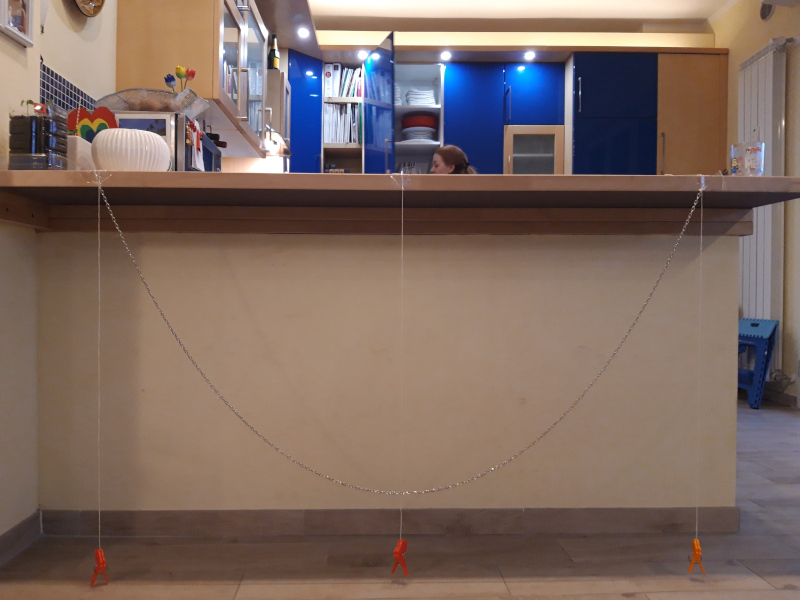
\includegraphics[width=\linewidth]{figures/catenaria}
\end{figure}

\labsubsection{Analisi dell'immagine}

Per misurare le coordinate dei punti di interesse potete aprire l'immagine in
matplotlib (come illustrato nell'esempio alla pagina seguente), posizionanddo il
mouse sui punti stessi e leggendo le coordinate sulla barra inferiore della
finestra. Se preferite, esiste un certo numero di alternative viabili, tra cui
l'utilizzo di un qualsiasi programma di manipolazione di immagini
(e.g., \url{https://www.gimp.org/}) oppure di una utility apposita come
\url{https://automeris.io/WebPlotDigitizer/}.

Notate che, in questo modo, tutte le vostre coordinate saranno espresse in
\emph{pixel}. Per convertire (e misurare il parametro $a$) in unit\`a fisiche
avrete bisogno di ricavare il fattore si scala corrispondente a partire da un
elemento di lunghezza nota nella vostra immagine.

Fate attenzione alla stima delle incertezze di misura. Se siete sicuri di
riuscire ad identificare con sicurezza il pixel corrispondente al punto di
interesse, potete assumere che la misura sia \emph{digitale}, con una risoluzione
di 1~pixel. Ma quali sono i fattori che potrebbero invalidare questa assunzione?


\labsubsection{Fit e grafico dei residui}

Una volta eseguito il fit, potete valutare l'accordo tra modello e dati
attraverso l'esame del grafico dei residui:
\begin{align}
  r_i = y_i - \mathcal{C}(x; \hat{a}, \hat{x_0}, \hat{y0}) \quad \text{e}
  \quad \sigma_{r_i} = \sigma_{y_i}.
\end{align}
Se il modello, valutato in corrispondenza dei parametri di \emph{best fit},
fornisce una buona descrizione dei dati, allora i residui debbono oscillare
intorno allo zero con fluttuazioni paragonabili all'ampiezza delle barre
d'errore. Qualsiasi deviazione indica un potenziale problema con il modello o
con la stima delle incertezze (o entrambe).

Cosa concludete dall'analisi del grafico dei residui?


\secconsiderations

Si consiglia di scegliere una corda (o una catena) con una densit\`a lineare
non troppo piccola, ma allo stesso tempo quanto pi\`u possibile flessibile
(e, ovviamente, omogenea). Sperimentate diverse soluzioni per trovare quella che
fa al caso vostro.

La parte pi\`u difficoltosa dell'esperienza sar\`a probabilmente  il riuscire a
scattare una foto con un angolazione tale da evitare deformazioni significative
nel piano della corda. A questo scopo potete aiutarvi con due o pi\'u di fili a
piombo---o addirittura con una griglia disegnata su un foglio di carta ed appesa
opportunemente sullo sfondo (che vi aiuterebbe anche nella conversione tra
pixel ed unit\`a fisiche).

Nella stesura della relazione siete caldamente incoraggiati ad essere prodighi
di dettagli sul \emph{setup} sperimentale che avete usato (e.g., foto) e a
mettere in evidenza le difficolt\`a che avete incontrato nella misura
(e gli accorgimenti che avete utilizzato per superarle).

\onecolumn

\begin{Verbatim}[label=\makebox{\href{https://github.com/unipi-physics-labs/lab1-sheets/tree/main/snippy/dad_catenaria.py}{https://github.com/.../dad\_catenaria.py}},commandchars=\\\{\}]
\PY{k+kn}{import}\PY{+w}{ }\PY{n+nn}{numpy}\PY{+w}{ }\PY{k}{as}\PY{+w}{ }\PY{n+nn}{np}
\PY{k+kn}{import}\PY{+w}{ }\PY{n+nn}{matplotlib}
\PY{k+kn}{from}\PY{+w}{ }\PY{n+nn}{matplotlib}\PY{+w}{ }\PY{k+kn}{import} \PY{n}{pyplot} \PY{k}{as} \PY{n}{plt}
\PY{k+kn}{from}\PY{+w}{ }\PY{n+nn}{scipy}\PY{n+nn}{.}\PY{n+nn}{optimize}\PY{+w}{ }\PY{k+kn}{import} \PY{n}{curve\PYZus{}fit}

\PY{c+c1}{\PYZsh{} Visualizzazione dell\PYZsq{}immagine in matplotlib\PYZhy{}\PYZhy{}\PYZhy{}va da se\PYZsq{}: dovete sostituire il}
\PY{c+c1}{\PYZsh{} percorso al file contenente l\PYZsq{}immagine con quello appropriato per voi.}
\PY{c+c1}{\PYZsh{} Una volta aperta l\PYZsq{}immagine in matplotlib potete andare sopra con il mouse e}
\PY{c+c1}{\PYZsh{} vedrete la posizione (in pixel) visualizzata sulla barra inferiore della finestra.}
\PY{c+c1}{\PYZsh{} Questo vi permette di misurare manualmente la posizione di un numero arbitrario}
\PY{c+c1}{\PYZsh{} di punti nell\PYZsq{}immagine stessa.}
\PY{n}{file\PYZus{}path} \PY{o}{=} \PY{l+s+s1}{\PYZsq{}}\PY{l+s+s1}{../figures/catenaria.jpg}\PY{l+s+s1}{\PYZsq{}}
\PY{n}{plt}\PY{o}{.}\PY{n}{figure}\PY{p}{(}\PY{l+s+s1}{\PYZsq{}}\PY{l+s+s1}{Immagine originale}\PY{l+s+s1}{\PYZsq{}}\PY{p}{)}
\PY{n}{img} \PY{o}{=} \PY{n}{matplotlib}\PY{o}{.}\PY{n}{image}\PY{o}{.}\PY{n}{imread}\PY{p}{(}\PY{n}{file\PYZus{}path}\PY{p}{)}
\PY{n}{plt}\PY{o}{.}\PY{n}{xlabel}\PY{p}{(}\PY{l+s+s1}{\PYZsq{}}\PY{l+s+s1}{x [pixels]}\PY{l+s+s1}{\PYZsq{}}\PY{p}{)}
\PY{n}{plt}\PY{o}{.}\PY{n}{ylabel}\PY{p}{(}\PY{l+s+s1}{\PYZsq{}}\PY{l+s+s1}{y [pixels]}\PY{l+s+s1}{\PYZsq{}}\PY{p}{)}
\PY{n}{plt}\PY{o}{.}\PY{n}{imshow}\PY{p}{(}\PY{n}{img}\PY{p}{)}

\PY{k}{def}\PY{+w}{ }\PY{n+nf}{catenary}\PY{p}{(}\PY{n}{x}\PY{p}{,} \PY{n}{a}\PY{p}{,} \PY{n}{c}\PY{p}{,} \PY{n}{x0}\PY{p}{)}\PY{p}{:}
\PY{+w}{    }\PY{l+s+sd}{\PYZdq{}\PYZdq{}\PYZdq{}Modello di catenaria.}
\PY{l+s+sd}{    \PYZdq{}\PYZdq{}\PYZdq{}}
    \PY{k}{return} \PY{n}{c} \PY{o}{+} \PY{n}{a} \PY{o}{*} \PY{n}{np}\PY{o}{.}\PY{n}{cosh}\PY{p}{(}\PY{p}{(}\PY{n}{x} \PY{o}{\PYZhy{}} \PY{n}{x0}\PY{p}{)} \PY{o}{/} \PY{n}{a}\PY{p}{)}

\PY{c+c1}{\PYZsh{} Come prima: usate il percorso al vostro file.}
\PY{n}{file\PYZus{}path} \PY{o}{=} \PY{l+s+s1}{\PYZsq{}}\PY{l+s+s1}{../macro/data/catenaria.txt}\PY{l+s+s1}{\PYZsq{}}
\PY{n}{x}\PY{p}{,} \PY{n}{y} \PY{o}{=} \PY{n}{np}\PY{o}{.}\PY{n}{loadtxt}\PY{p}{(}\PY{n}{file\PYZus{}path}\PY{p}{,} \PY{n}{unpack}\PY{o}{=}\PY{k+kc}{True}\PY{p}{)}
\PY{c+c1}{\PYZsh{} Ricordate: il riferimento delle immagini, tipicamente, e` in alto a sinistra,}
\PY{c+c1}{\PYZsh{} per cui potreste aver bisogno di cambiare segno alla y.}
\PY{n}{y} \PY{o}{=} \PY{o}{\PYZhy{}}\PY{n}{y}
\PY{c+c1}{\PYZsh{} Fate attenzione alle incertezze: il valore, qui, e` completamente arbitario.}
\PY{n}{sigma\PYZus{}y} \PY{o}{=} \PY{l+m+mf}{3.}

\PY{c+c1}{\PYZsh{} Grafico principale.}
\PY{n}{fig} \PY{o}{=} \PY{n}{plt}\PY{o}{.}\PY{n}{figure}\PY{p}{(}\PY{l+s+s1}{\PYZsq{}}\PY{l+s+s1}{Fit e residui}\PY{l+s+s1}{\PYZsq{}}\PY{p}{)}
\PY{n}{fig}\PY{o}{.}\PY{n}{add\PYZus{}axes}\PY{p}{(}\PY{p}{(}\PY{l+m+mf}{0.1}\PY{p}{,} \PY{l+m+mf}{0.3}\PY{p}{,} \PY{l+m+mf}{0.8}\PY{p}{,} \PY{l+m+mf}{0.6}\PY{p}{)}\PY{p}{)}
\PY{n}{plt}\PY{o}{.}\PY{n}{errorbar}\PY{p}{(}\PY{n}{x}\PY{p}{,} \PY{n}{y}\PY{p}{,} \PY{n}{sigma\PYZus{}y}\PY{p}{,} \PY{n}{fmt}\PY{o}{=}\PY{l+s+s1}{\PYZsq{}}\PY{l+s+s1}{o}\PY{l+s+s1}{\PYZsq{}}\PY{p}{)}
\PY{c+c1}{\PYZsh{} Fit. Notate che, per far convergere il fit, avrete bisogno di fornire una}
\PY{c+c1}{\PYZsh{} stima iniziale ragionevole dei parametri.}
\PY{n}{popt}\PY{p}{,} \PY{n}{pcov} \PY{o}{=} \PY{n}{curve\PYZus{}fit}\PY{p}{(}\PY{n}{catenary}\PY{p}{,} \PY{n}{x}\PY{p}{,} \PY{n}{y}\PY{p}{,} \PY{n}{p0}\PY{o}{=}\PY{p}{(}\PY{l+m+mf}{1000.}\PY{p}{,} \PY{o}{\PYZhy{}}\PY{l+m+mf}{3000.}\PY{p}{,} \PY{l+m+mf}{2300.}\PY{p}{)}\PY{p}{)}
\PY{n}{a\PYZus{}hat}\PY{p}{,} \PY{n}{c\PYZus{}hat}\PY{p}{,} \PY{n}{x0\PYZus{}hat} \PY{o}{=} \PY{n}{popt}
\PY{n}{sigma\PYZus{}a}\PY{p}{,} \PY{n}{sigma\PYZus{}c}\PY{p}{,} \PY{n}{sigma\PYZus{}x0} \PY{o}{=} \PY{n}{np}\PY{o}{.}\PY{n}{sqrt}\PY{p}{(}\PY{n}{pcov}\PY{o}{.}\PY{n}{diagonal}\PY{p}{(}\PY{p}{)}\PY{p}{)}
\PY{n+nb}{print}\PY{p}{(}\PY{n}{a\PYZus{}hat}\PY{p}{,} \PY{n}{sigma\PYZus{}a}\PY{p}{,} \PY{n}{c\PYZus{}hat}\PY{p}{,} \PY{n}{sigma\PYZus{}c}\PY{p}{,} \PY{n}{x0\PYZus{}hat}\PY{p}{,} \PY{n}{sigma\PYZus{}x0}\PY{p}{)}
\PY{n}{plt}\PY{o}{.}\PY{n}{plot}\PY{p}{(}\PY{n}{x}\PY{p}{,} \PY{n}{catenary}\PY{p}{(}\PY{n}{x}\PY{p}{,} \PY{n}{a\PYZus{}hat}\PY{p}{,} \PY{n}{c\PYZus{}hat}\PY{p}{,} \PY{n}{x0\PYZus{}hat}\PY{p}{)}\PY{p}{)}
\PY{n}{plt}\PY{o}{.}\PY{n}{grid}\PY{p}{(}\PY{n}{which}\PY{o}{=}\PY{l+s+s1}{\PYZsq{}}\PY{l+s+s1}{both}\PY{l+s+s1}{\PYZsq{}}\PY{p}{,} \PY{n}{ls}\PY{o}{=}\PY{l+s+s1}{\PYZsq{}}\PY{l+s+s1}{dashed}\PY{l+s+s1}{\PYZsq{}}\PY{p}{,} \PY{n}{color}\PY{o}{=}\PY{l+s+s1}{\PYZsq{}}\PY{l+s+s1}{gray}\PY{l+s+s1}{\PYZsq{}}\PY{p}{)}
\PY{n}{plt}\PY{o}{.}\PY{n}{ylabel}\PY{p}{(}\PY{l+s+s1}{\PYZsq{}}\PY{l+s+s1}{y [u. a.]}\PY{l+s+s1}{\PYZsq{}}\PY{p}{)}
\PY{c+c1}{\PYZsh{} Grafico dei residui.}
\PY{n}{fig}\PY{o}{.}\PY{n}{add\PYZus{}axes}\PY{p}{(}\PY{p}{(}\PY{l+m+mf}{0.1}\PY{p}{,} \PY{l+m+mf}{0.1}\PY{p}{,} \PY{l+m+mf}{0.8}\PY{p}{,} \PY{l+m+mf}{0.2}\PY{p}{)}\PY{p}{)}
\PY{n}{res} \PY{o}{=} \PY{n}{y} \PY{o}{\PYZhy{}} \PY{n}{catenary}\PY{p}{(}\PY{n}{x}\PY{p}{,} \PY{n}{a\PYZus{}hat}\PY{p}{,} \PY{n}{c\PYZus{}hat}\PY{p}{,} \PY{n}{x0\PYZus{}hat}\PY{p}{)}
\PY{n}{plt}\PY{o}{.}\PY{n}{errorbar}\PY{p}{(}\PY{n}{x}\PY{p}{,} \PY{n}{res}\PY{p}{,} \PY{n}{sigma\PYZus{}y}\PY{p}{,} \PY{n}{fmt}\PY{o}{=}\PY{l+s+s1}{\PYZsq{}}\PY{l+s+s1}{o}\PY{l+s+s1}{\PYZsq{}}\PY{p}{)}
\PY{n}{plt}\PY{o}{.}\PY{n}{grid}\PY{p}{(}\PY{n}{which}\PY{o}{=}\PY{l+s+s1}{\PYZsq{}}\PY{l+s+s1}{both}\PY{l+s+s1}{\PYZsq{}}\PY{p}{,} \PY{n}{ls}\PY{o}{=}\PY{l+s+s1}{\PYZsq{}}\PY{l+s+s1}{dashed}\PY{l+s+s1}{\PYZsq{}}\PY{p}{,} \PY{n}{color}\PY{o}{=}\PY{l+s+s1}{\PYZsq{}}\PY{l+s+s1}{gray}\PY{l+s+s1}{\PYZsq{}}\PY{p}{)}
\PY{n}{plt}\PY{o}{.}\PY{n}{xlabel}\PY{p}{(}\PY{l+s+s1}{\PYZsq{}}\PY{l+s+s1}{x [u. a.]}\PY{l+s+s1}{\PYZsq{}}\PY{p}{)}
\PY{n}{plt}\PY{o}{.}\PY{n}{ylabel}\PY{p}{(}\PY{l+s+s1}{\PYZsq{}}\PY{l+s+s1}{Residuals}\PY{l+s+s1}{\PYZsq{}}\PY{p}{)}
\PY{n}{plt}\PY{o}{.}\PY{n}{ylim}\PY{p}{(}\PY{o}{\PYZhy{}}\PY{l+m+mf}{20.0}\PY{p}{,} \PY{l+m+mf}{20.0}\PY{p}{)}
\PY{n}{plt}\PY{o}{.}\PY{n}{savefig}\PY{p}{(}\PY{l+s+s1}{\PYZsq{}}\PY{l+s+s1}{catenaria.pdf}\PY{l+s+s1}{\PYZsq{}}\PY{p}{)}

\PY{n}{plt}\PY{o}{.}\PY{n}{show}\PY{p}{(}\PY{p}{)}
\end{Verbatim}



\end{article}
\end{document}
